\documentclass[12pt]{article} 
\usepackage{amsmath} 
\usepackage[dvips]{graphicx}
\usepackage{multirow} 
\usepackage{geometry} 
\usepackage{pdflscape}
\usepackage[labelfont=bf]{caption} 
\usepackage{setspace}
\usepackage[running]{lineno} 
% \usepackage[numbers,sort]{natbib}
\usepackage[round]{natbib} 
\usepackage{array}
\usepackage[table]{xcolor}
\usepackage{xr}

\newcommand{\methods}{\textit{Materials \& Methods}}
\newcommand{\SI}{\textit{Appendix}~}

\topmargin -1.5cm % 0.0cm 
\oddsidemargin 0.0cm % 0.2cm 
\textwidth 6.5in
\textheight 9.0in % 21cm
\footskip 1.0cm % 1.0cm

\usepackage{authblk}

\begin{document} 

\title{Do motif roles provide unique information about species risk of extinction?\\ \medskip Supplementary Information}


\author{Anna \r{A}kesson$^{1\dagger}$, Alyssa R. Cirtwill$^{2}$, Kate Wootton$^{3}$, Gyuri Barab\'{a}s$^{1}$, Anna Ekl\"{o}f$^{1}$} 
\date{\small$^1$Department of Theoretical Biology, Chemistry, and Physics\\ 
Link\"{o}ping University\\
Link\"{o}ping, Sweden\\
\medskip
\small$^2$Department of Agricultural Sciences\\
University of Helsinki\\
Helsinki, Finland\\
\medskip
\small$^3$ University of Colorado?\\
\medskip
$^\dagger$ Corresponding author:\\
}



\maketitle 
\raggedright

\setlength{\parindent}{15pt} 
\begin{spacing}{2.0}

\clearpage

\section*{Table of contents}
    \begin{spacing}{1.0}

    \begin{enumerate}
    
        \item How do counts of motifs in a network profile vary with S and C? \\
        
            \begin{itemize}
            \item Same methods as main text except using counts instead of proportions to define motif profiles
            \end{itemize}
            
            
        \item Motif profiles differed slightly between network sets

           \begin{itemize}
                \item Comparing proportions of motifs in un-filtered, filtered, and acyclic networks.
                \item AFAIK not referred to in text
            \end{itemize}    
            
        
         \item Persistence and count-based motif participation

           \begin{itemize}
                \item Should be as main text section 4, but counts
            \end{itemize}
                
        
        \item Motif-persistence relationships and network size
            \begin{itemize}
                \item Detailed results for variability of slopes for persistence $\approx$ motif participation in networks of different sizes.
                \item Main text refers to C, moved figure to Main while we check that we've got everything.
            \end{itemize}


        \item How does persistence vary with degree and trophic level?

            \begin{itemize}
                \item Heat map showing persistence vs. TL with BP=0
                \item Heat map showing persistence vs. TL with BP=1
            \end{itemize}
    
    \end{enumerate}
\end{spacing}
\clearpage

   
\section{How do counts of motifs in a network profile vary with S and C?} 

    
    As expected, all four motifs had higher counts in larger and more highly connected networks.
    The precise effects of size, connectance, and their interaction differed between motifs  (Table~\ref{network_motif_lms}).
    This suggests that the meso-scale structure of a network varies with size and connectance, not just the total number of motifs.
    Indeed, the motif profile of a network is significantly related to its size, connectance, and their interaction ($F_{1,2996}$=2279, $p$\textless0.001; $F_{1,2996}$=3067, $p$\textless0.001; and $F_{1,2996}$=1187, $p$\textless0.001, respectively).


    \begin{table}[h!]
        \centering
        \caption{Coefficients for linear regressions relating the total count of all motifs or the count of each three-species motif in a network to network size, connectance, and their interaction. Coefficients in \textbf{bold} are significant (\textless0.05). Note that, while there are 13 unique three-species motifs, only four are possible in acyclic networks such as those considered here.}
       \label{network_motif_lms}
       \begin{tabular}{c|c c c c c}
        Motif & Intercept & Size & Connectance & Interaction \\
        \hline
        Total count & \textbf{-2.85$\times10^3$} & \textbf{46.6} & \textbf{-2.12$\times10^{5}$} & \textbf{4.72$\times10^{3}$} \\
        \hline
        Thee-species Chain & \textbf{-1.40$\times10^{3}$} & \textbf{26.1} & \textbf{-3.74$\times10^{4}$} & \textbf{8.58$\times10^{2}$} \\
        Apparent Competition & \textbf{-2.23$\times10^3$} & \textbf{42.0} & 
        \textbf{-7.26$\times10^4$} & \textbf{1.63$\times10^3$} \\
        Direct Competition & 26.6 & 0.777 & \textbf{-4.85$\times10^4$} & \textbf{9.89$\times10^2$} \\
        Omnivory & \textbf{7.57} & \textbf{-22.2} & \textbf{-5.37$\times10^4$} & \textbf{1.24$\times10^3$} \\
        \hline
        \end{tabular}
    \end{table}
    
        
    \begin{figure}[h!]
        \centering
        \includegraphics[width=.75\textwidth]{figures/motif_profile_dispersion.pdf}
        \caption{Dispersion of motif profiles within a network about the centroid for that combination of network size and connectance. Each circle represents a single network; circle colour indicates network size. Scatter has been introduced about each level of connectance to increase visual clarity; the levels of connectance we consider are indicated by vertical black lines.}
        \label{dispersion_rawmotifs}
    \end{figure}

    
    Motif profiles were similarly variable across networks with different sizes, but were not homogeneously variable across connectances or size-connectance combinations ($F_{5,2994}$=0.365, $p$=0.873; $F_{4,2995}$=4.49, $p$=0.001; and $F_{29,2970}$=27.1, $p$\textless0.001 , respectively).
    These differences in variability of motif profiles can cause false positives in the PERMANOVA.
    Variability in motif profiles was lowest among large networks with moderate connectance and was highest among the least-connected and most-connected networks we considered (Fig.~\ref{dispersion_rawmotifs}).


    \begin{figure}[h!]
        \centering
        \includegraphics[width=\textwidth]{figures/absolute_lmer_allCS.pdf}
        \caption{The effect of number of times a species appears (x-axis) in any of the various motifs (columns) on persistence (y-axis). The effect of each motif participation is fitted by linear mixed-effect models, following Equation~\ref{absreq}, except that the disturbance levels are fitted separately. The different colored lines indicate various disturbances on the basal level, from $\pi_{disturbed} = 0.1$ (in the top) to $\pi_{disturbed} = 0.5$ (in the bottom).}
        \label{fig:abs_lmer_all}
    \end{figure}            


\clearpage


\section{Motif profiles differed slightly in different network sets}

    Not all motifs were equally likely to occur in the networks we considered. 
    Across the initially stable, acyclic networks (i.e., those used in the main text), the omnivory motif tended to make up a smaller proportion of the motif profile than other motifs.
    The omnivory motif was also rarer than the three-species chain and apparent competition motifs before networks were rendered acyclic, but made up a similar proportion to the direct competition motif (Table~\ref{tab:acyclic_proportions}).
    The omnivory motif made up a larger proportion of the full set of initially stable networks, including those which were excluded from our final analysis due to overly high trophic levels.
    Nevertheless, in each group of networks the apparent competition and three-species chain motifs made up the largest proportion of the motif profile.
    This suggests that, while rendering networks acyclic does change proportions slightly, stable networks created by the niche model appear to be generally biased towards the chain and apparent competition motifs.
    
    \begin{table}[h!]
        \centering
        \caption{Proportions of the four motifs which appear in Bayesian networks (three-species chain: `Chain', apparent competition: `AC', direct competition `DC', and omnivory: `Omni') and other motifs (`Other') in the motif profiles of acyclic, filtered, and original networks. Acyclic networks are those used in the main text analyses. Filtered networks are those used in the main text analyses \emph{before} being rendered acyclic. Original networks are all simulated networks, including those removed because of overly high maximum trophic levels.}
        \label{tab:acyclic_proportions}            \footnotesize
        \begin{tabular}{c|l l l | l l l | l l l |}
        & \multicolumn{3}{c|}{Acyclic networks} & \multicolumn{3}{c|}{Filtered networks} & \multicolumn{3}{c|}{Original networks} \\
        Motif & Mean (SD) & Min & Max & Mean (SD) & Min & Max & Mean (SD) & Min & Max \\
        \hline
        Chain & 0.235 (0.042) & 0.109 & 0.412 & 0.225 (0.045) & 0.100 & 0.412 & 0.218 (0.043) & 0.096 & 0.413 \\
        AC & 0.422 (0.064) & 0.250 & 0.765 &
        0.417 (0.067) & 0.233 & 0.765 & 0.397 (0.064) & 0.231 & 0.765 \\
        DC & 0.179 (0.041) & 0.050 & 0.359 & 0.155 (0.046) & 0.040 & 0.359 & 0.140 (0.046) & 0.031 & 0.359 \\
        Omni & 0.164 (0.079) & 0.006 & 0.346 & 0.156 (0.075) & 0.006 & 0.319 & 0.184 (0.073) & 0.006 & 0.329 \\
        \hline
        Other & \multicolumn{3}{c|}{NA} & 0.047 (0.042) & 0.00 & 0.200 &
        0.062 (0.046) & 0.00 & 0.258 \\
        \end{tabular}
    \end{table}

\clearpage

\section{Persistence and count-based motif participation}

    \subsection*{Methods}

        We test whether participating in higher absolute numbers (i.e., counts) of a motif increases persistence using a set of models that parallels those used to test whether having a greater proportion of the role made up by a particular motif (see \emph{Main Text}).  
        Specifically, we fit four linear mixed-effect models (LMMs; one per motif included in the Bayesian networks).
        In each case, we considered only non-basal species (i.e., those with at least one prey) as the persistence of basal species is determined only by their baseline probability.
        These models included the absolute number of times the focal species appeared in the focal motif, the increase in probability of extinction for basal species, and the interaction between the two as well as a random intercept for the interaction between species richness and connectance (equations.
        All models were fit using the R~\citep{R} function `lmer' from the package \emph{lmerTest}~\citep{lmerTest}.
        We calculated marginal (fixed effects only) and conditional (fixed and random effects) $R^2$ using the R~\citep{R} function `r.squaredGLMM' from the package \emph{MuMIn}~\citep{MuMIn}.

            The formula for these LMMs are:         
            \begin{equation}
                \Psi_{ik} \approx \chi_{i} + \pi_{disturbed_k} + \chi_{i}\pi_{disturbed_k} + S:C_{i} ,
                \label{absreq}
            \end{equation}
        
            \noindent where $\Psi_ik$ is the persistence of species $i$ during disturbance level $k$, $\chi_{i}$ is the number of times species $i$ appears in the focal motif, $\pi_{disturbed_k}$ is the probability of extinction for a basal resource in disturbance level $k$, and $S:C_{i}$ is a random intercept for the species richness and connectance of the network containing species $i$.
            
            
            % Additionally, we performed a similar linear regression of persistence against motif participation within each simulated network and for each level of disturbance to basal resources (XX regressions total).
            % These regressions were fit using the R~\citep{R} base function `lm'.
            % We then analyse the distribution of slopes for the effect of motif participation across levels of disturbance, network size, and connectance.  
            

    \subsection*{Results}

        \begin{figure}[h!]
            \centering
            \includegraphics[width=\textwidth]{figures/absolute_lmer_allCS.pdf}
            \caption{The effect of number of times a species appear (x-axis) in any of the various motifs (columns) on persistence (y-axis). The effect of each motif participation is fitted by linear mixed-effect models, following \emph{Equation 2; Main Text}, except that the disturbance levels are fitted separately. The different colored lines indicate various disturbances on the basal level, from $\pi_{disturbed} = 0.1$ (in the top) to $\pi_{disturbed} = 0.5$ (in the bottom).}
            \label{fig:abs_lmer_all}
        \end{figure}            
    
    
        Persistence increased significantly with the number of times a species appeared in any of the four possible motifs in the food webs (Table~\ref{tab:absolute_number} and Figure~\ref{fig:abs_lmer_all}). 
        These relationships were slightly stronger for the number of times a species appears in the three-species chain and direct competition motifs and somewhat weaker for apparent competition and omnivory. The absolute difference between the motifs was small, with a clear positive relationship between persistence and motif count present in all cases. 
        As expected, persistence decreased significantly with increasing disturbance of basal resources and the strength of this relationship was very similar across the four motifs.
        The level of disturbance to basal resources also affected the relationship between persistence and motif counts.
        For all four motifs, there was a negative interaction between motif count and disturbance such that, for high levels of disturbance, participating more often in any of the motifs would result in decreased persistence.
    
        \begin{table}[h!]
            \caption{Coefficients ($\beta$) for models relating persistence to the number of times a species appears in the focal motif, the level of disturbance to basal resources, and their interaction, as well as a random intercept to account for differences in persistence across levels of network size and connectance (Equation~\ref{absreq}). $p$-values for all coefficients in all models were \textless0.001. We also provide the marginal $R^2_M$ (fixed effects only) and conditional $R^2_C$ (fixed and random effects) for each model.}
            \label{tab:absolute_number}        \centering
            \begin{tabular}{c|c  c c  c | c c |}
            Motif & Intercept & Motif count & Disturbance & Interaction & $R^2_M$ & $R^2_C$ \\
            \hline
            3-sp Chain & 0.762 & 1.14$\times10^{-4}$ & -0.388 & -1.36$\times10^{-4}$ & 0.897 & 0.913 \\
            Apparent Compet. & 0.770 & 3.41$\times10^{-5}$ & -0.397 & -4.36$\times10^{-5}$ & 0.898 & 0.911\\
            Direct Competition & 0.764 & 1.22$\times10^{-4}$ & -0.398 & -8.46$\times10^{-5}$ & 0.895 & 0.914 \\
            Omnivory & 0.770 & 6.01$\times10^{-5}$ & -0.400 & -5.91$\times10^{-5}$ & 0.897 & 0.912 \\                
            \end{tabular}
            \end{table}
                
\clearpage
           
\section{Motif-persistence relationships and network size}

    When comparing the outcomes from linear mixed-effect models (LMMs) relating persistence to motif roles across all networks (Fig. 3 and Table 1, \emph{Main Text}) with similar linear regressions (LRs) made on each single network separately, the main trends are similar but different-sized networks showed slightly different results results for some motifs (Figure temporarily in main text).%(Figure~\ref{fig:density_prop_S}). 
    For the three-species chain and omnivory motifs, a significant interaction between disturbance and the effect of the focal motif means that having a larger proportion of the role be made up of the chain or omnivory motif is associated with lower persistence at high levels of disturbance (Fig. 3 and Table 1, \emph{Main Text}). 
    The same pattern holds overall for LRs fit within a network  %(Figure~\ref{fig:density_prop_S})
    : the fraction of negative slopes for the proportion of three-species chain and omnivory motifs increases with increasing disturbance. 
    This trend is most pronounced in large networks.% (bottom panel, Figure~\ref{fig:density_prop_S}). 
    Besides the decrease in fraction of positive slopes with increasing disturbance, the omnivory motif show a higher overall fraction of positive slopes in comparison to the three-species chain motif, corresponding to the positive main effect of omnivory (Fig. 3 and Table 1, \emph{Main Text}). 


    % \begin{figure}[h!]
    %      \centering
    %      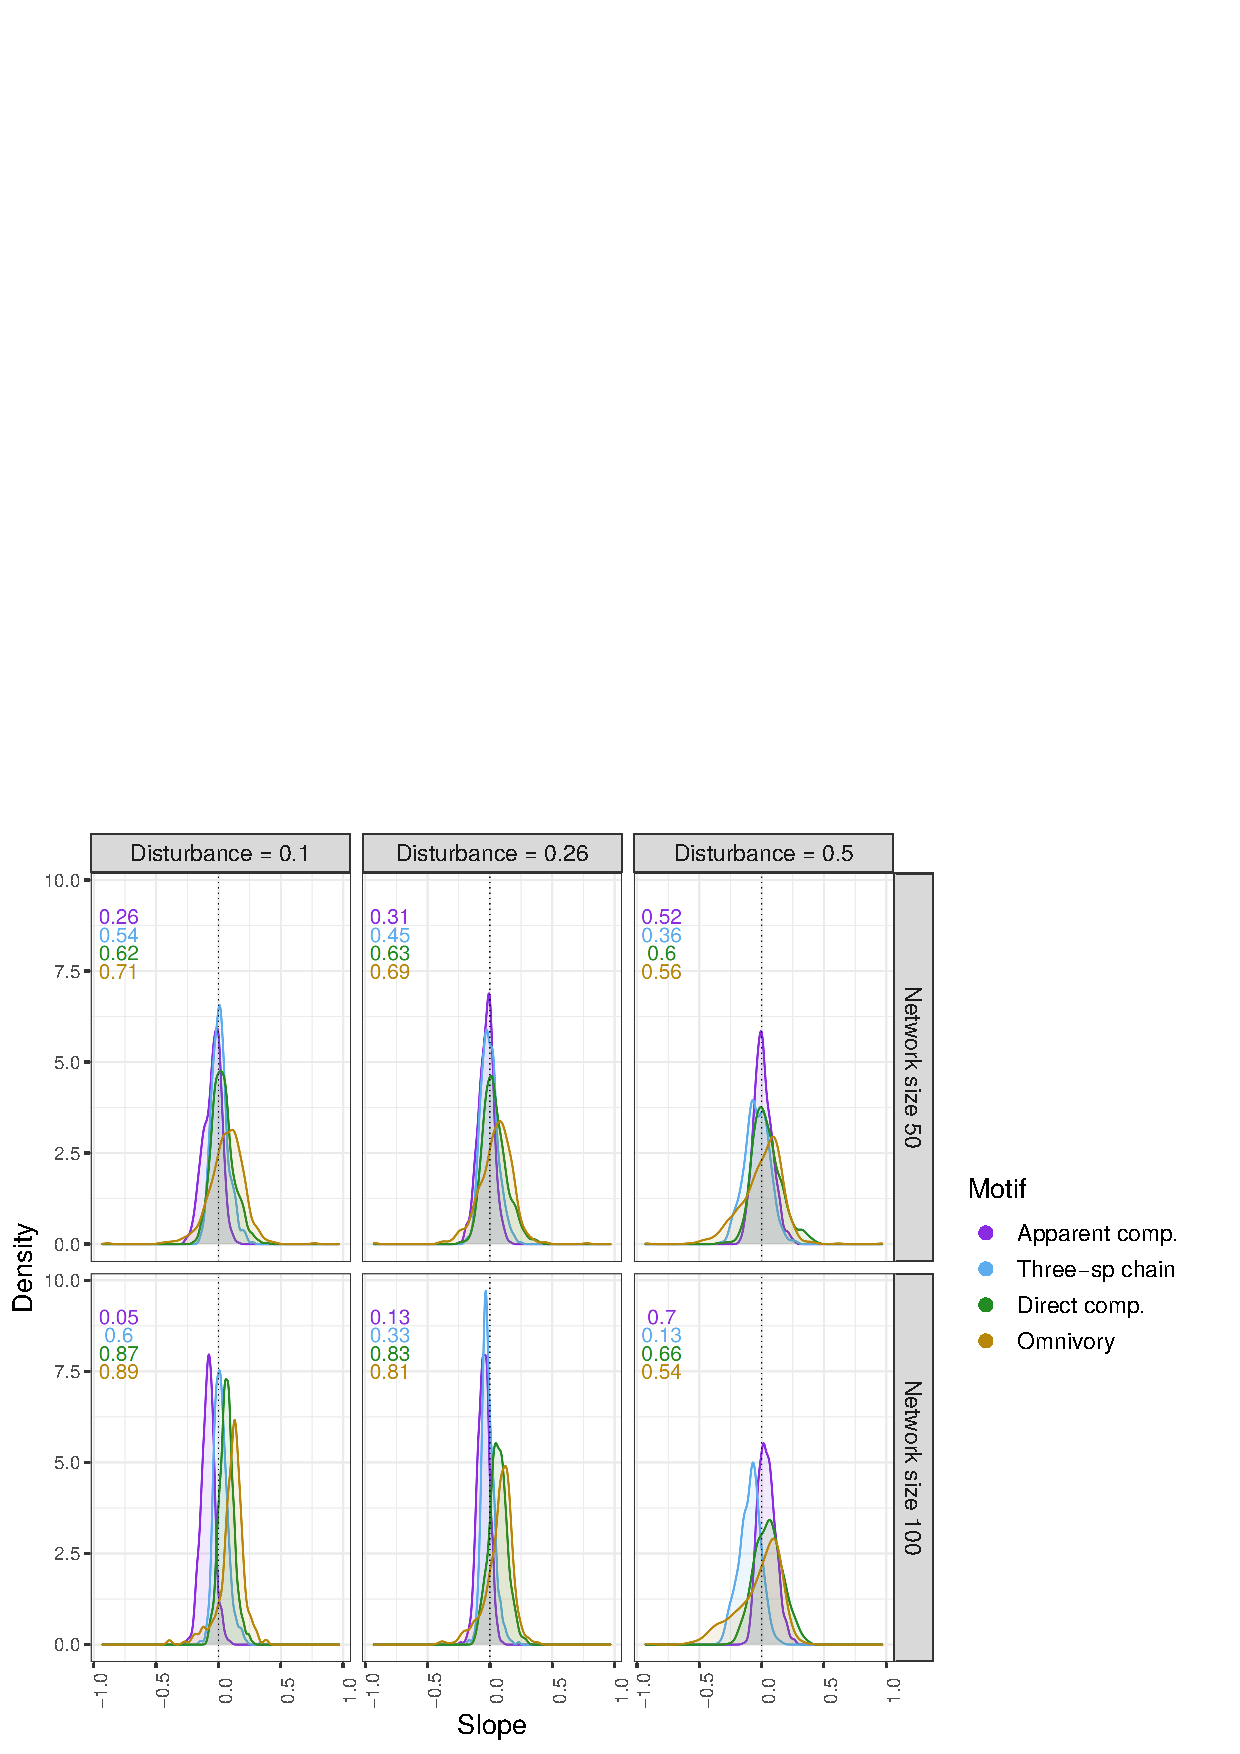
\includegraphics[width=\textwidth]{manuscript/figures/prop_dens_bp_vs_S_allC.pdf}
    
    %     \caption{Density (y-axis) of slopes (x-axis) for all simulated webs of all sizes - a visualization of how an increased proportion of each motif (different colored lines) affects persistence of consumer species. The slopes are derived from linear mixed-effect models, with a random intercept for the interaction between species richness and network size. A negative slope value reflects a negative relationship between increased participation in a motif and persistence, while a positive slope value reflects a positive relationship - an increased proportion of a specific motif increase persistence. The fraction of replicates with a slope greater than zero are stated in numbers in each sub-plot, the color corresponding to motif (legend). Columns show the result for various disturbances on the basal level, from $\pi_{disturbed} = 0.1$ (left) to $\pi_{disturbed} = 0.5$ (right). Rows show various levels of network size. The vertical line indicate zero on the x-axis.}
    %     \label{fig:density_prop_S}
    % \end{figure}
    
    
    For the apparent and direct competition motifs, the LMMs include a positive interaction between disturbance and the proportion of the motif in a species' role (Fig. 3 and Table 1; \emph{Main Text}).
    This means that having more of the role made up of these two motifs is increasingly beneficial at higher levels of disturbance, a trend which is also evident from the increasing fraction of positive slopes with increasing disturbance based on LRs of each network at each level of disturbance. % (Figure~\ref{fig:density_prop_S}).
    As with the trends for omnivory and three-species chains, these increases are strongest in large networks. % (bottom row, Figure~\ref{fig:density_prop_S}).
    % For direct competition, the fraction of slopes are similar across disturbance levels. Although this interaction is not positive when accounting for network size, the fraction of positive slopes are throughout high.
    The increase in the proportion of positive slopes was much stronger for apparent competition than direct competition, consistent with the smaller (but still significant) interaction term for between direct competition in the LMMs.
    A high proportion of direct competition in a species' role tended to be associated with greater probability of persistence across levels of disturbance and network size.
    % In conclusion, species richness does not considerably alter the trends visible in the LMMs. High species richness more clearly display an interaction between motif proportion, persistences and disturbance levels, while this effect is smaller with low species richness. 
                
            

\section{How does persistence vary with degree and trophic level?}

  \begin{figure}
     \centering
     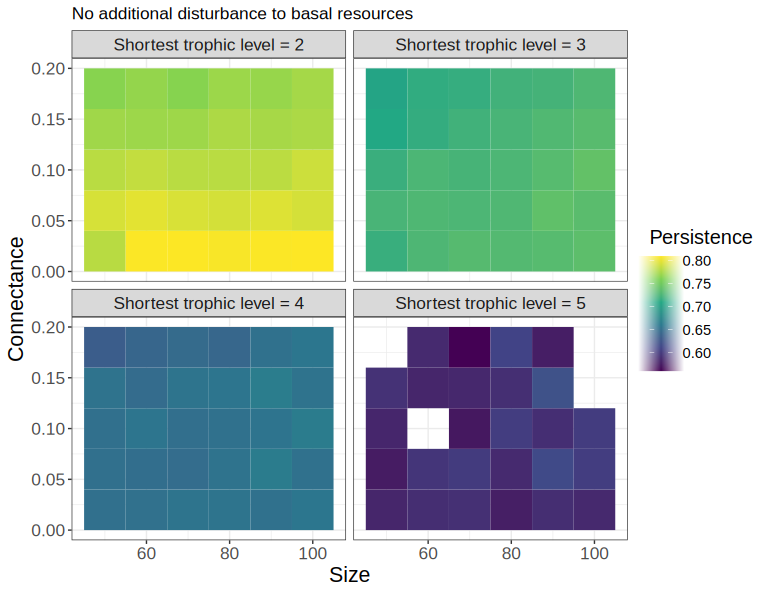
\includegraphics[width=0.8\textwidth]{figures/heatmap_STL_allCS_BP0.pdf}
    
     \caption{All species across all levels experience a risk of going extinct due to causes not related to the web of $\pi = 0.1$. The sub figures show final persistence for consumers with different shortest trophic length, for increasing connectance (y-axis) and network size (x-axis). Persistence decreases with darker color in the heat map.}
     \label{fig:heatmap_stl_BP0}
 \end{figure}

 \begin{figure}
     \centering
     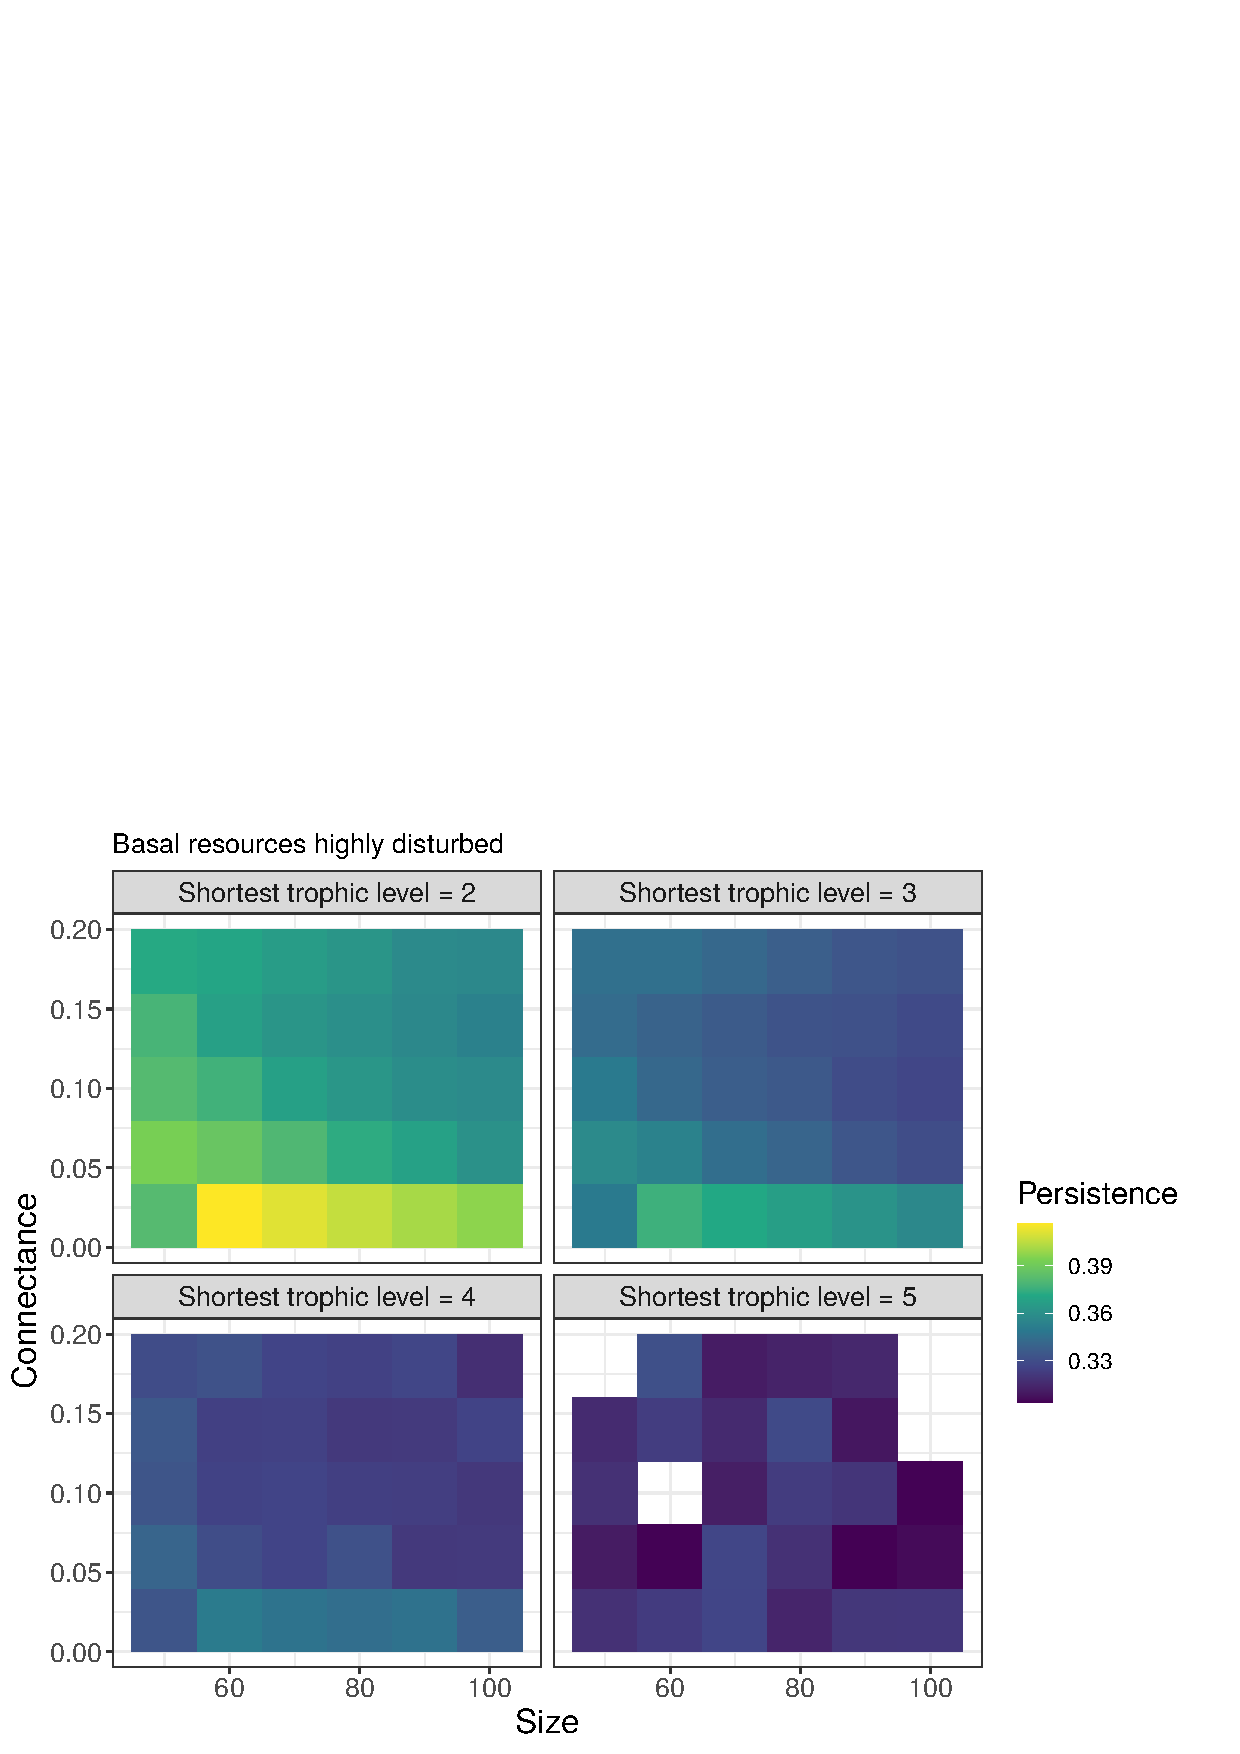
\includegraphics[width=0.8\textwidth]{figures/heatmap_STL_allCS_BP1.pdf}
    
     \caption{Primary producers experience a disturbance reducing their probability to go extinct to $\pi_{disturbed} = 0.5$ All consumer species go extinct due to causes not related to the web itself with probability $\pi = 0.1$. The sub figures show final persistence for consumers with different shortest trophic length, for increasing connectance (y-axis) and network size (x-axis). Persistence decreases with darker color in the heat map.}
     \label{fig:heatmap_stl_BP1}
 \end{figure}

\clearpage 
\bibliographystyle{ecollett} 
\bibliography{MyCollection} % Abbreviate journal titles.

\end{spacing}

\end{document}